\section{Member}
\begin{center}\begin{tabular}{ |c| } \hline Name \\ \hline Lin Zhi Jie \\ \hline Kang Chih Yung \\ \hline Li Guan Hao \\ \hline \end{tabular}\end{center}

\section{Introduction}
Our project is a game that use funny buttons to reach the goal unmber.
\section{Design Viewpoints}

\subsection{Logical Viewpoint}

\subsubsection{Background Class}
Background Class will show background.
\begin{center}\begin{tabular}{ |c| } \hline Background \\ \hline -int: height \\ -int: width \\ \hline +Background() \\ +getHeight() \\ +getWidth() \\ +setHeight(int height) \\ +setWidth(int width) \\ \hline \end{tabular}\end{center}

\subsubsection{Button Class}
Button Class will allow users to click.
\begin{center}\begin{tabular}{ |c| } \hline Button \\ \hline -int: height \\ -int: width \\ \hline +Button() \\ +getHeight() \\ +getWidth() \\ +setHeight(int height) \\ +setWidth(int width) \\ \hline \end{tabular}\end{center}

\subsubsection{Main Menu Button Class}
Main Menu Button Class will allow users to enter Level Menu From Main Menu.
\begin{center}\begin{tabular}{ |c| } \hline Main Menu Button \\ \hline +MainMenuButton() \\ +GoLevelMenu()\\ \hline \end{tabular}\end{center}

\subsubsection{Main Menu Background Class}
Main Menu Class will show users main menu. 
\begin{center}\begin{tabular}{ |c| } \hline Main Menu Background \\ \hline -Menu Button: Start \\ \hline +MainMenu() \\ \hline \end{tabular}\end{center}

\subsubsection{Level List Button Class}
Level List Button Class will offer users to enter chosen level.
\begin{center}\begin{tabular}{ |c| } \hline Level List Button \\ \hline -static int: total \\ -int: id \\ \hline +LevelListButton() \\ +GoLevel() \\ \hline \end{tabular}\end{center}

\subsubsection{Level Menu Background Class}
Level Main Menu Class will show users levels.
\begin{center}\begin{tabular}{ |c| } \hline Level Menu Background \\ \hline -Level List Button[]: LevelListButtons \\ \hline +LevelMenu() \\ \hline \end{tabular}\end{center}

\subsubsection{Modify Button Class}
Modify Button Class will change state in level.
\begin{center}\begin{tabular}{ |c| } \hline Level List Button \\ \hline String: description\\ \hline +ModifyButton() \\ \hline \end{tabular}\end{center}

\subsubsection{Level Background Class}
Level Class will show level and allow user to play it.
\begin{center}\begin{tabular}{ |c| } \hline Level \\ \hline -int: id \\ -int: state \\ -int: goal \\ -int: move \\ -Modify Button[]: ModifyButtons \\ \hline +LevelBackground() \\ \hline \end{tabular}\end{center}
\subsection{Extend Viewpoint}
\subsubsection{Background Extend}
\begin{figure}[H]
\graphicspath{{pic/}}
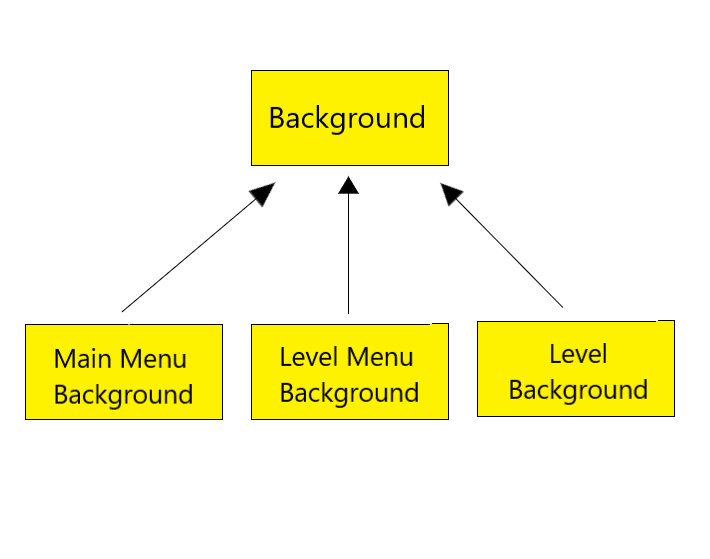
\includegraphics[scale=0.5]{bg.png}
\caption{Background Extend}
\vskip 0pt
\end{figure}

\subsubsection{Button Extend}

\begin{figure}[H]
\graphicspath{{pic/}}
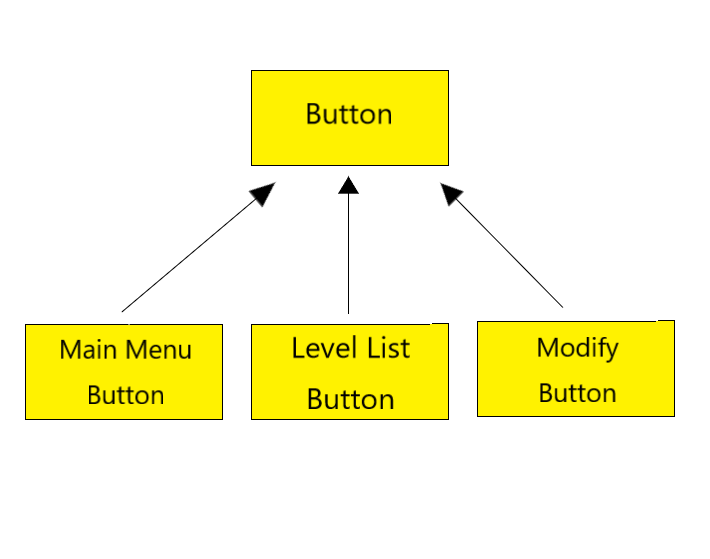
\includegraphics[scale=0.5]{button.png}
\caption{Button Extend}
\vskip 0pt
\end{figure}